%                                                                 aa.dem
% AA vers. 8.2, LaTeX class for Astronomy & Astrophysics
% demonstration file
%                                                       (c) EDP Sciences
%-----------------------------------------------------------------------
%
%\documentclass[referee]{aa} % for a referee version
%\documentclass[onecolumn]{aa} % for a paper on 1 column  
%\documentclass[longauth]{aa} % for the long lists of affiliations 
%\documentclass[rnote]{aa} % for the research notes
%\documentclass[letter]{aa} % for the letters 
%\documentclass[bibyear]{aa} % if the references are not structured 
% according to the author-year natbib style

%
\documentclass[referee]{aa}  
\usepackage{natbib}
\bibpunct{(}{)}{;}{a}{}{,} % to follow the A&A style

%
\usepackage{graphicx}
%%%%%%%%%%%%%%%%%%%%%%%%%%%%%%%%%%%%%%%%
\usepackage{txfonts}
%%%%%%%%%%%%%%%%%%%%%%%%%%%%%%%%%%%%%%%%
%\usepackage[options]{hyperref}
% To add links in your PDF file, use the package "hyperref"
% with options according to your LaTeX or PDFLaTeX drivers.
%
\begin{document} 


   \title{JUICE-ExPRES}

   \subtitle{}

   \author{B. Cecconi
          \inst{1}
          \and
          C. Louis\inst{2}
          }

   \institute{LESIA, Observatoire de Paris, CNRS, PSL Research University, Meudon, France\\
              \email{baptiste.Cecconi@observatoiredeparis.psl.eu}
         \and
             IRAP, CNRS, Université Paul Sabatier, Toulouse, France\\
             \email{corentin.louis@irap.omp.eu}
             }

   \date{}

% \abstract{}{}{}{}{} 
% 5 {} token are mandatory
 
  \abstract
  % context heading (optional)
  % {} leave it empty if necessary  
   {}
  % aims heading (mandatory)
   {}
  % methods heading (mandatory)
   {}
  % results heading (mandatory)
   {}
  % conclusions heading (optional), leave it empty if necessary 
   {}

   \keywords{Radio emissions --
                Jupiter -- 
                JUICE mission
               }

   \maketitle
%
%________________________________________________________________

\section{Introduction}

The Jovian radio emissions
JUICE 

Jovian radio emissions

ExPRES \citep{Louis_AA_2019}   

%__________________________________________________________________

\section{Jovian radio emissions occultation by Ganymede}
\citet{kurth_GRL_97} observed that the Jovian hectometric radio emissions are occulted by Ganymede during G01 flyby (first Ganymede flyby) of the Galileo S/C, on June 27th 1996. Figure \ref{fig:g01} shows the Galileo/PWS (Plasma Waves Science) \citep{gurnett_SSR_92} spectrogram during G01 flyby. The occultation is observed between 05:50 and 06:20 SCET. The occultation spectral ingress and egress profiles imply that radio sources at higher frequencies (located close to Jupiter) are occulted earlier and reappears later than the lower frequency sources (located further out from Jupiter).

We model this occultation using ExPRES. The location of the visible radio sources is modeled every minute of time during the interval displayed on Figure \ref{fig:g01}. Northern and Southern main auroral oval are modeled with active magnetic field lines every 1$^\circ$ on longitude.  We use the JRM09 magnetic field model \citep{Connerney:2018jx} and the magnetic latitude of the active magnetic field lines correspond to $L_\textrm{shell}=30$ \citep{Grodent:2015eo}. The unstable electron temperature set to 5~keV \citep{Louarn:2017bc}. 

The occultation is computed using a simple computation of the intercept distance between the center of Ganymede and the straight lines passing by each radio source and the observer. The occultation estimation uses a simple occultation by the surface of Ganymede: any source with an intercept distance shorter than one Ganymede Radius is occulted, as sketched on Figure \ref{fig:occult}.

%The second occultation estimation includes a model of the Ganymede's ionosphere (e.g., as in Eviatar et al (2001)), and uses the modeled cutoff frequency altitude for each frequency.

\begin{figure}
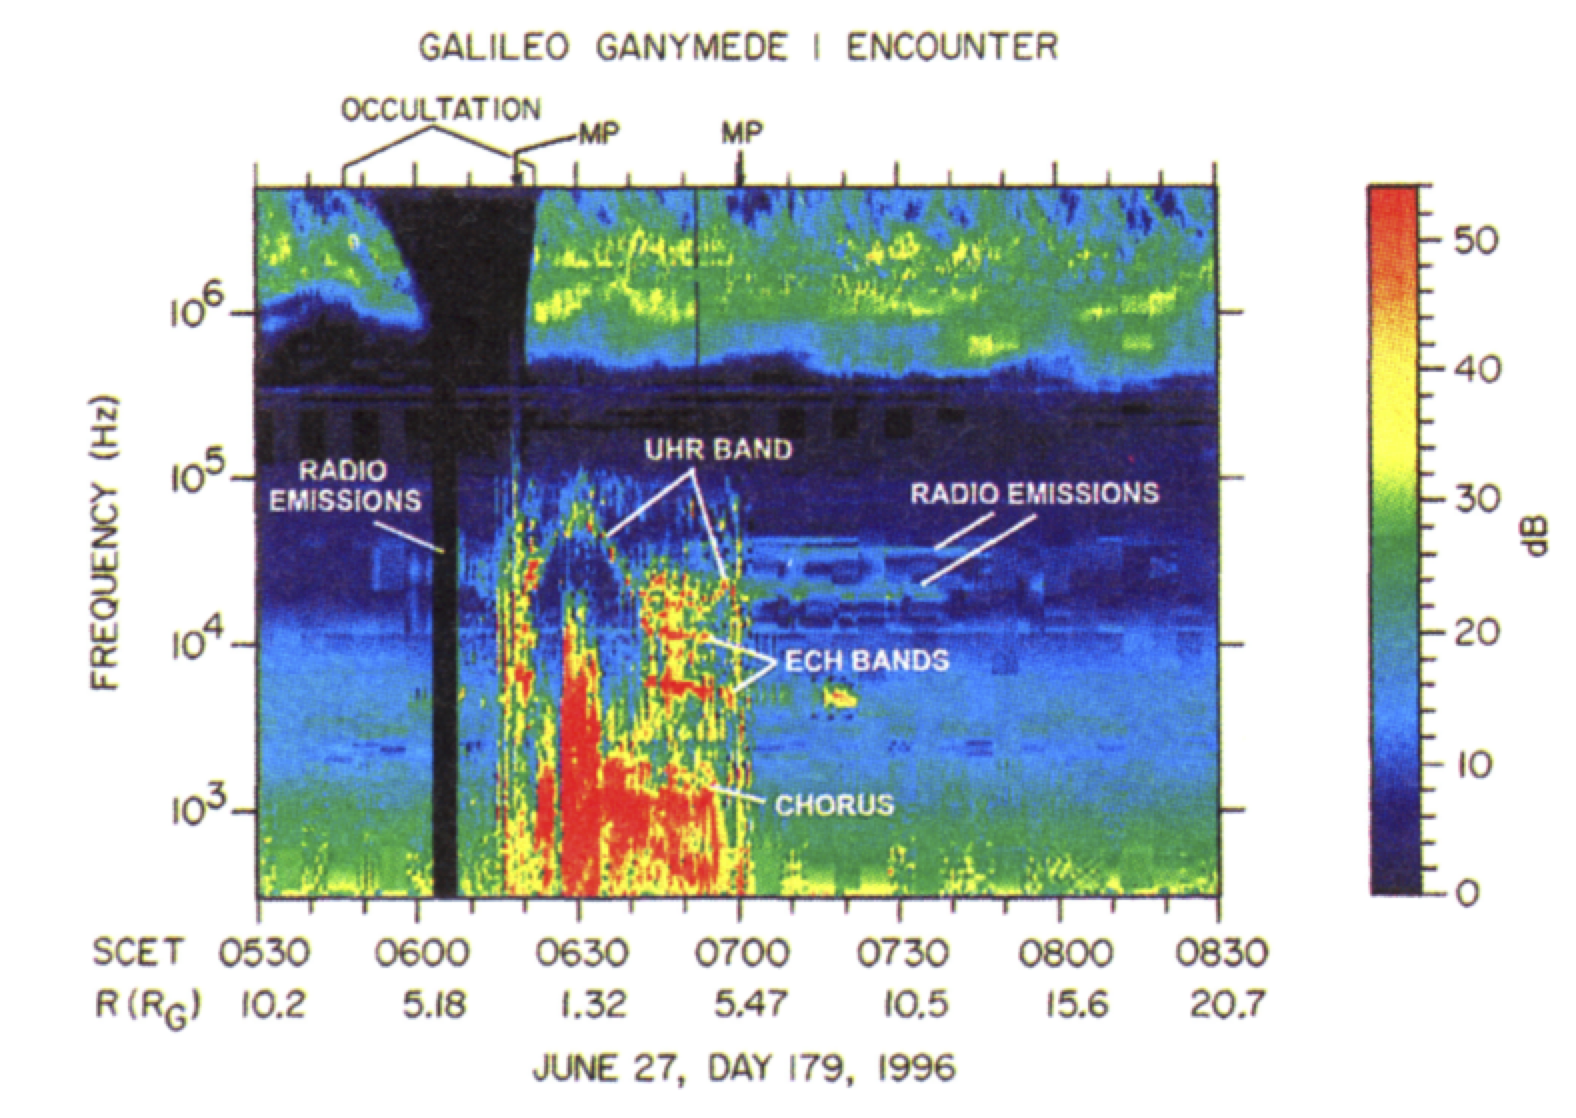
\includegraphics[width=\linewidth]{gll-g01.png}
\caption{Galileo PWS spectrogram observed during G01 flyby. The Jovian radio emissions are visible at }\label{fig:g01}
\end{figure}

\begin{figure}
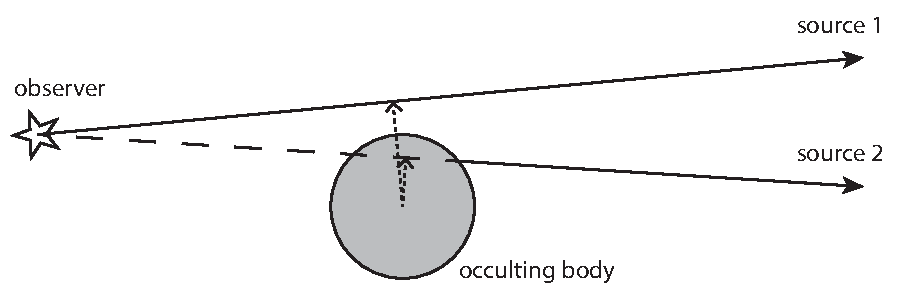
\includegraphics[width=0.7\linewidth]{occult.pdf}
\caption{Simple geometrical occultation scheme used in this study. The intercept distance (dotted segment) is computed as the distance between the center of occulting body (here, Ganymede), and the straight line passing by each radio source and the observer.}\label{fig:occult}
\end{figure}

\bibliographystyle{aa}
\bibliography{juice-expres}
\end{document}
